\documentclass[a4paper,11pt]{article}
\usepackage{ls}
%\usepgfplotslibrary{patchplots}
\pgfplotsset{compat=newest} 

\pagestyle{empty}
\begin{document}

\begin{center}
    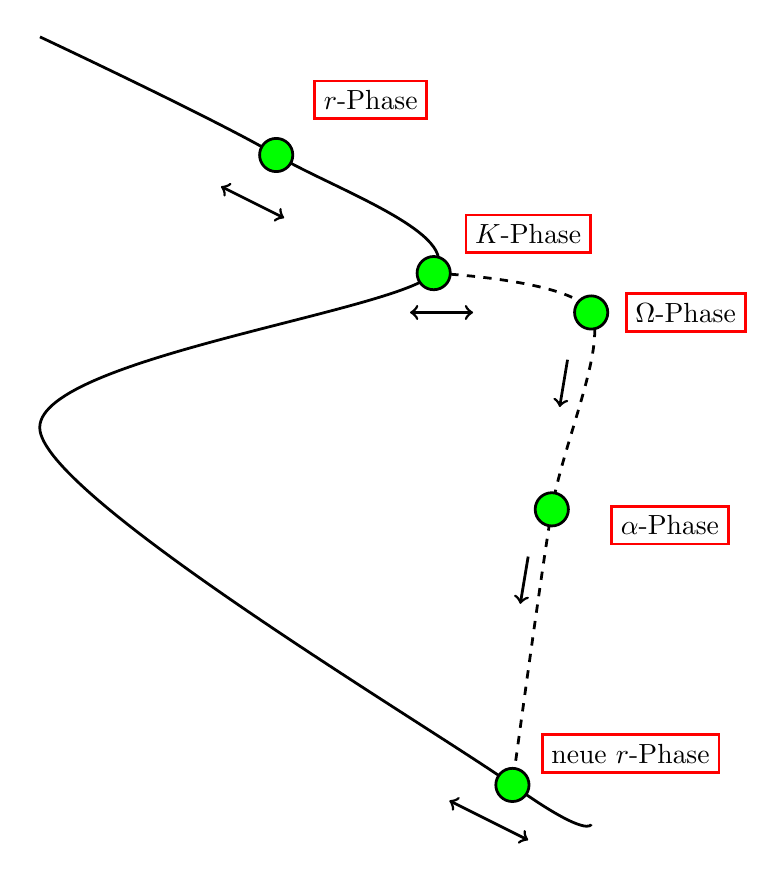
\begin{tikzpicture}[line width=1pt,transform shape]
    \node (A0) at (0,10) {};
    \node (A4) at (3,8.5) {};
    \node (A1) at (5,7) {};
    \node (A1a) at (7,6.5) {};
    \node (A2) at (0,5) {};
    \node (A3) at (7,0) {};
    \node (A5) at (6.5,4) {};
    \node (A6) at (6,.5) {};
    \draw plot [smooth] coordinates {(A0) (A4) (A1) (A2) (A6) (A3)};
    \node[draw=red] at (4.2,9.2) [rectangle] {$r$-Phase};
    \draw[<->] (2.3,8.1) -- (3.1,7.7) ;
    \node[draw=red] at (6.2,7.5) [rectangle] {$K$-Phase};
    \draw[<->] (4.7,6.5) -- (5.5,6.5) ;
    \node[draw=red] at (8.2,6.5) [rectangle] {$\Omega$-Phase};
    \draw[->] (6.7,5.9) -- (6.6,5.3) ;
    \node[draw=red] at (8,3.8) [rectangle] {$\alpha$-Phase};
    \draw[->] (6.2,3.4) -- (6.1,2.8) ;
    \draw[<->] (5.2,.3) -- (6.2,-.2) ;
    \draw[fill=green] (A4) circle (6pt) ;
    \draw[->,dashed] plot [smooth] coordinates {(A1) (A1a) (A5) (A6)};
    \draw[fill=green] (A1) circle (6pt) ;
    \draw[fill=green] (A1a) circle (6pt) ;
    \draw[fill=green] (A5) circle (6pt) ;
    \draw[fill=green] (A6) circle (6pt) ;
    \node[draw=red,fill=white] at (7.5,0.9) [rectangle] {neue $r$-Phase};
  \end{tikzpicture}
\end{center}
\end{document}

\begin{center}
  \begin{tikzpicture}[line width=1pt]
    \node[draw,text width=3em, align=center] [circle] (A0) {K};
    \node[draw,text width=2cm, align=center, above left=of A0] [rectangle] (I)
         {Input\\Blech}; 
    \node[draw,text width=2cm, align=center, above right=of A0] [rectangle] (O)
         {Output\\fertige\\Karosserie}; 
    \node[draw,below left=of A0, node distance=2em] [circle] (A1) {P};
    \node[draw,below right=of A0, node distance=2em] [circle] (A2) {L};
    \draw[->] (I)--(A0) ;
    \draw[->] (A0)--(O) ;
    \draw[->] (A0) to[bend right] (A1) ;
    \draw[->] (A1) to[bend right] (A0) ;
    \draw[->] (A0) to[bend right] (A2) ;
    \draw[->] (A2) to[bend right] (A0) ;
  \end{tikzpicture}
\end{center}

\begin{center}
  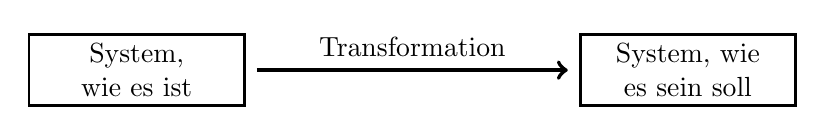
\begin{tikzpicture}[line width=1pt,
      pfeil/.style={shorten <=4pt, shorten >=4pt, line width=1.5pt},
      mytext/.style={text width=2.5cm,align=center}]
    \node[draw,mytext] at (0,0) [rectangle] (A0) {System, wie es ist};
    \node[draw,mytext] at (7,0) [rectangle] (A2) {System, wie es sein soll};
    \draw[pfeil,->] (A0)--(A2) ;
    \node[fill=white] at (3.5,.3) [rectangle] {Transformation};
  \end{tikzpicture}
\end{center}

\begin{center}
  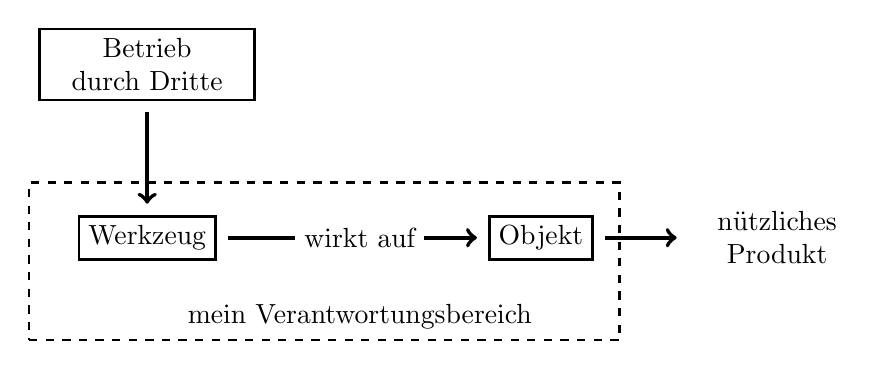
\begin{tikzpicture}[line width=1pt,
      pfeil/.style={shorten <=4pt, shorten >=4pt, line width=1.5pt},
      mytext/.style={text width=2.5cm,align=center}]
    \node[draw] at (0,1.3) [rectangle] (A0) {Werkzeug};
    \node[draw] at (5,1.3) [rectangle] (A2) {Objekt};
    \node[text width=2cm,align=center] at (8,1.3) [rectangle] (A3) {nützliches Produkt};
    \node[draw,mytext] at (0,3.5) [rectangle] (A4) {Betrieb durch Dritte};
    %\node[mytext,below of = A0] {Old state of the library};
    %\node[mytext,below of = A1] {New state of the library};
    \draw[pfeil,->] (A0)--(A2) ;
    \draw[pfeil,->] (A2)--(A3) ;
    \draw[pfeil,->] (A4)--(A0) ;
    \draw[dashed] (-1.5,0) -- (6,0) -- (6,2) -- (-1.5,2) -- cycle ;
    \node[fill=white] at (2.7,1.3) [rectangle] {wirkt auf};
    \node[] at (2.7,.3) {mein Verantwortungsbereich};
  \end{tikzpicture}
\end{center}
\end{document}

\begin{center}
  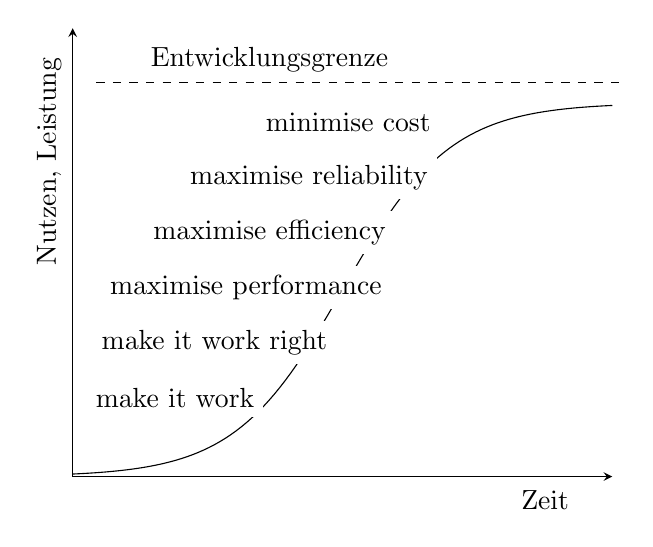
\begin{tikzpicture}
    \begin{axis}[
        xmin=0, xmax=10, ymin=0,ymax=12,
        axis lines=middle,
        xtick={\empty},ytick={\empty},
      ]
      \addplot[samples=100,domain=0:10] expression {10/(1+exp(-(x-5))) } ;
    \end{axis}
    \node[rotate=90] at (-.3,4) {Nutzen, Leistung} ;
    \node[] at (6,-.3) {Zeit} ;
    \node[] at (2.5,5.3) {Entwicklungsgrenze}; 
    \draw[-,dashed] (0.3,5) -- (7,5) ;
    \node[fill=white] at (1.3,1) {make it work} ;
    \node[fill=white] at (1.8,1.7) {make it work right} ;
    \node[fill=white] at (2.2,2.4) {maximise performance} ;
    \node[fill=white] at (2.5,3.1) {maximise efficiency} ;
    \node[fill=white] at (3,3.8) {maximise reliability} ;
    \node[fill=white] at (3.5,4.5) {minimise cost} ;
  \end{tikzpicture}\\[1em]
  Entwicklungsschritte entlang der S-Kurve am Beispiel Verbrennungsmotor
\end{center}
\end{document}
